
%\input{chapters/appendices/}
%\input{chapters/appendices/}

\chapter{Scripts and Code Snippets}

\section{Image Converter}
\lstinputlisting[firstline=14, label={code:imgConverter}, caption={Script to convert all images into a text file}]{../create_data.py}

\section{Image verification script}
\lstinputlisting[label={code:imgDisp}, caption={Data file displayer}, firstline=5]{../checkData.py}

\chapter{Images, figures and illustrations}

\begin{figure}[h]
\centering
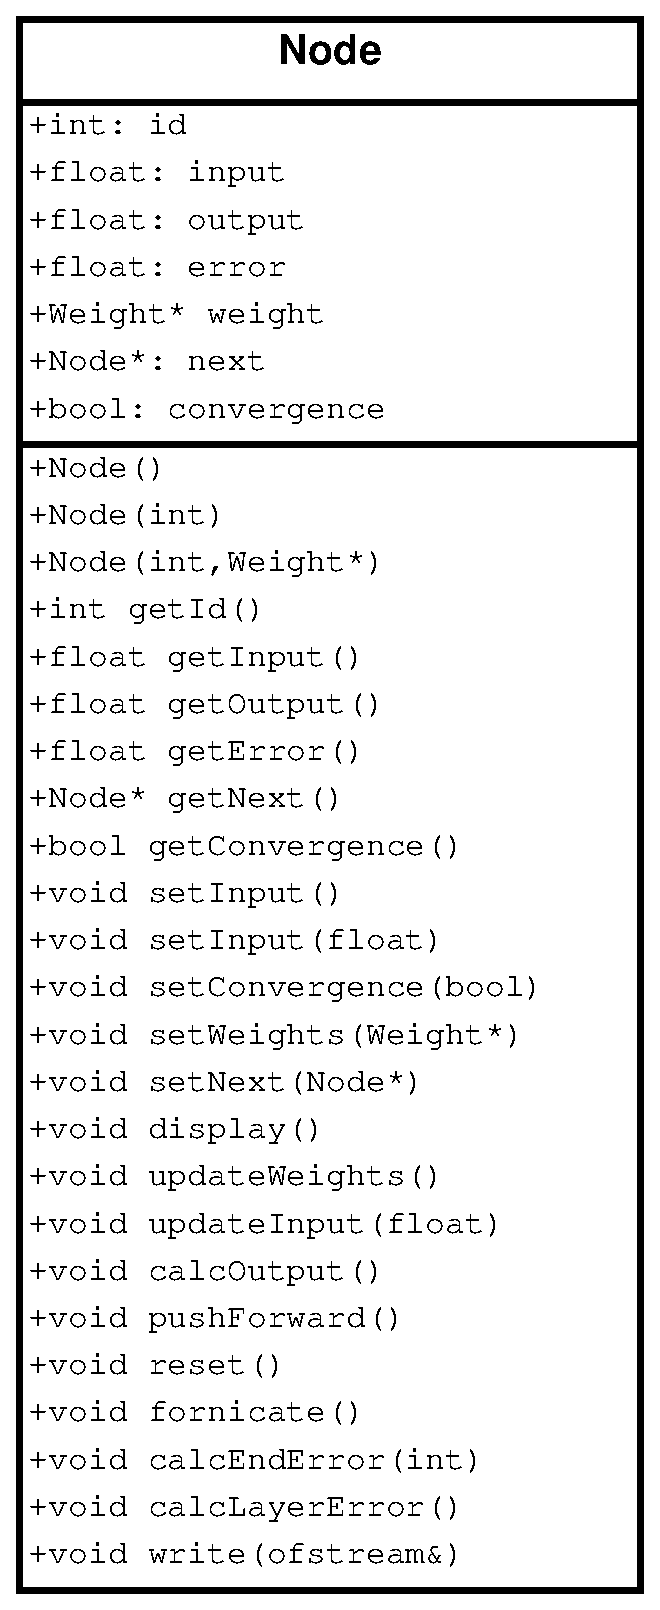
\includegraphics[width={0.4\textwidth}]{pictures/uml_node}
\caption{UML depiction of the perceptron}
\label{fig:uml_node}
\end{figure}

\begin{figure}[h]
\centering
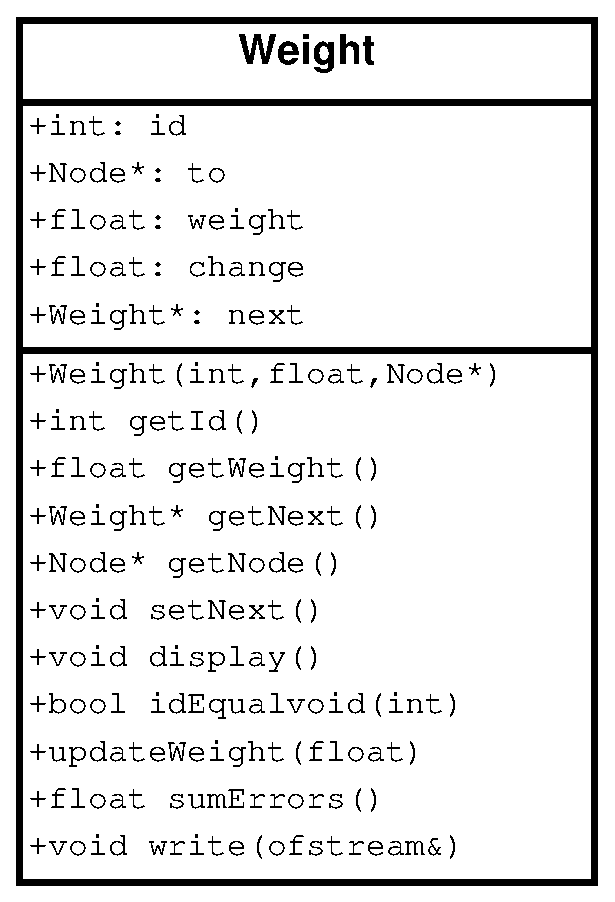
\includegraphics[width={0.4\textwidth}]{pictures/uml_weight}
\caption{UML depiction of the synapses}
\label{fig:uml_weight}
\end{figure}

\begin{figure}[h]
\centering
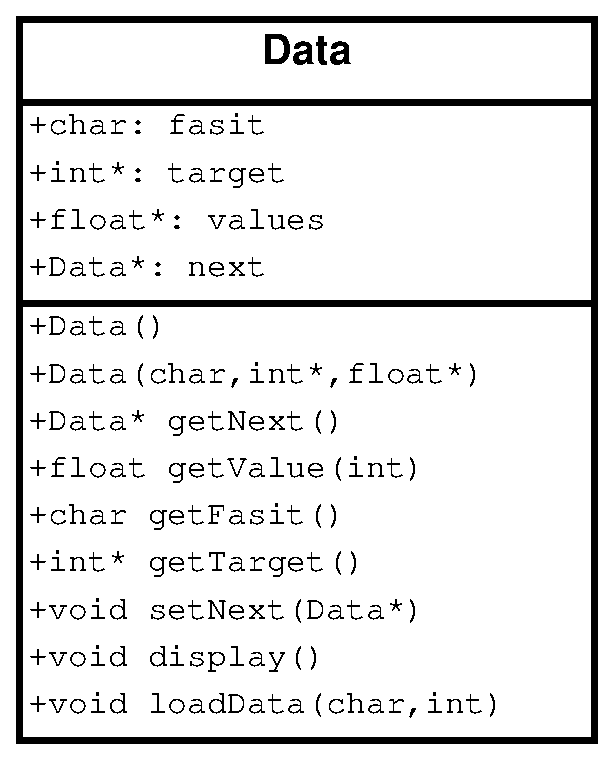
\includegraphics[width={0.4\textwidth}]{pictures/uml_data}
\caption{UML depiction of the image, data structure}
\label{fig:uml_data}
\end{figure}

\begin{figure}[h]
\centering
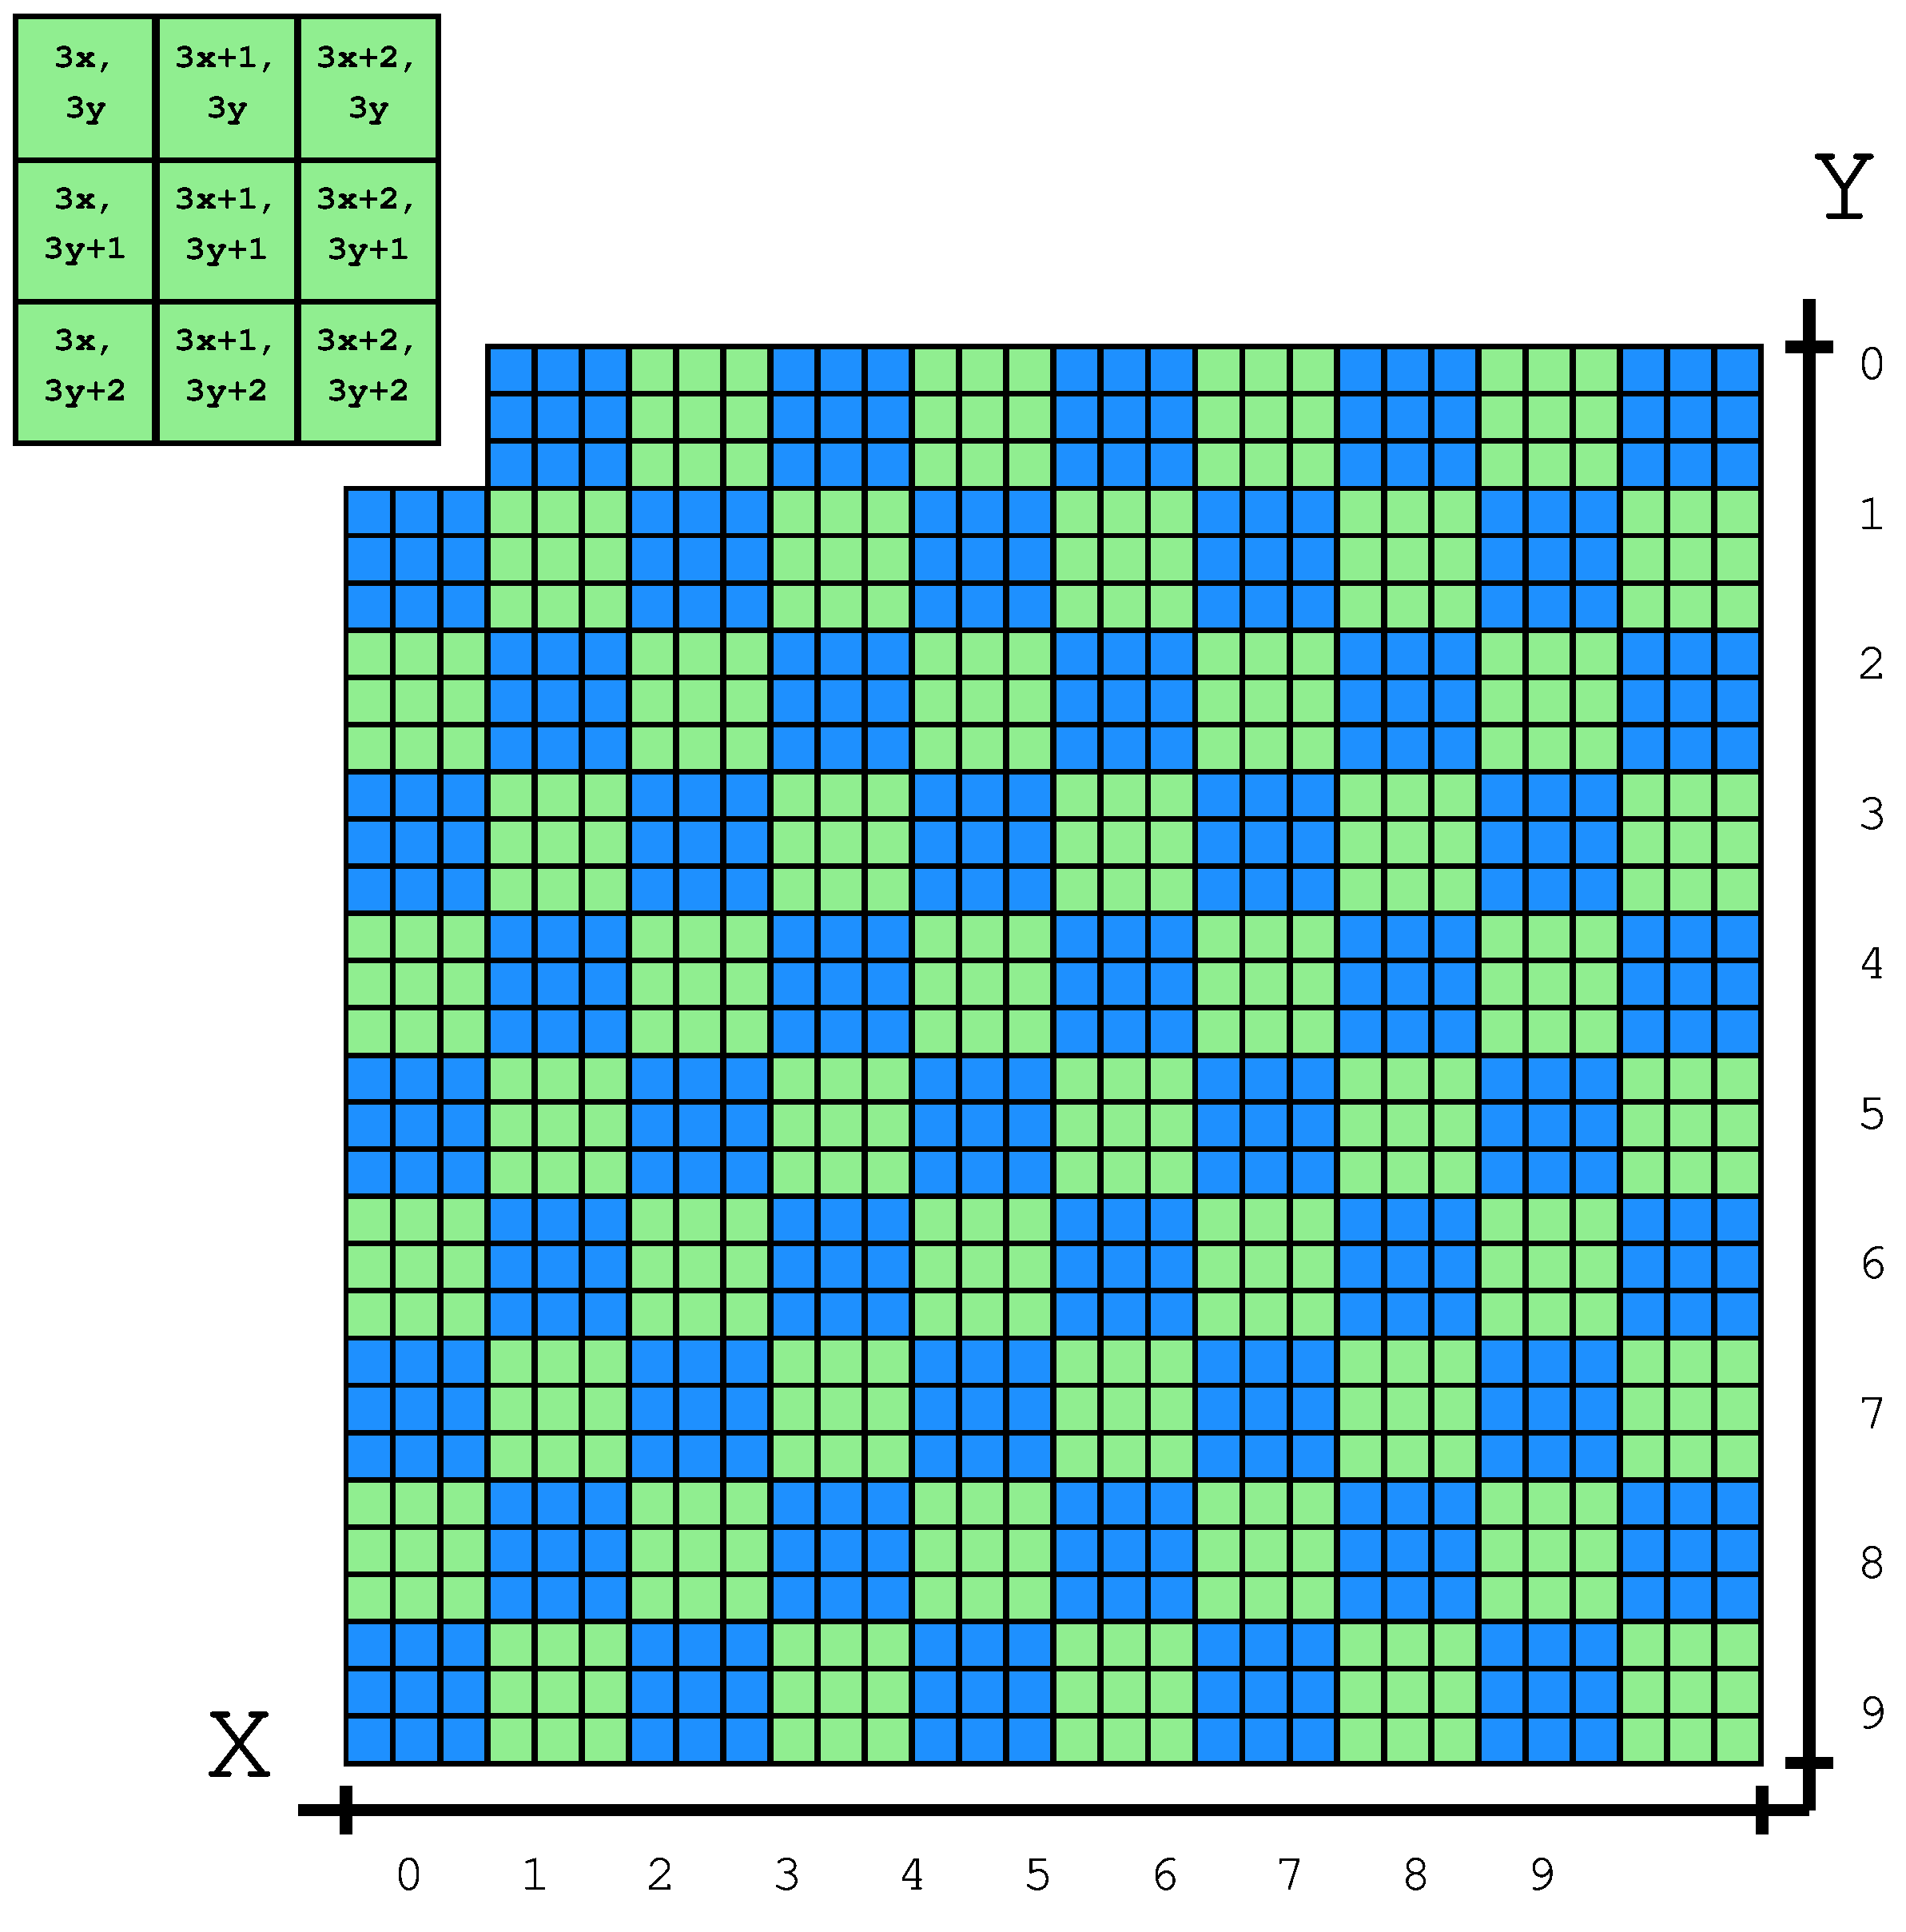
\includegraphics[width={1\textwidth}]{pictures/imgSubset}
\caption{How the image is divided into subsets and scaled down}
\label{fig:imgSubset}
\end{figure}


